\section{Results}
\label{sec:results_dilep}
A counting experiment (``cut-and-count analysis'') is performed in many bins across the \mZtwo spectrum to search for low-mass dilepton resonances~\cite{CMS:2021pcy}.
In the case of \htozdzd, where both of the daughter particles are identical, then a peak in the \mZtwo spectrum is expected at $(\mZone + \mZtwo) / 2$.
The \mZtwo distributions for the \htozzd and \htozdzd processes, categorized by the \mZtwo final states, can be seen in Figs.~\ref{fig:yield_hzzd_mZ2} and~\ref{fig:yield_hzdzd_mZ12}, respectively.
% 2\Pe and 2\Pmu final states are shown in Fig.~\ref{fig:yield_hzzd_mZ2} (A) and (B), respectively.
\begin{multiFigure}
    \centering
        \addFigure{0.48}{figures/dilep_res/yield_hzzd_mZ2_2mu.pdf}
        \addFigure{0.48}{figures/dilep_res/yield_hzzd_mZ2_2e.pdf}
    \captionof{figure}
        [Event yield within the distribution of \mZtwo in the \htozzd channel]
        {Event yield within the distribution of \mZtwo in the \htozzd channel.
        \;A) TODO
        \;B)}
    \label{fig:yield_hzzd_mZ2}
\end{multiFigure}
\begin{multiFigure}
    \centering
        \addFigure{0.48}{figures/dilep_res/yield_hzdzd_mZ12_4mu.pdf}
        \addFigure{0.48}{figures/dilep_res/yield_hzdzd_mZ12_4e.pdf}
        \addFigure{0.48}{figures/dilep_res/yield_hzdzd_mZ12_2e2mu.pdf}
    \captionof{figure}
        [Event yield within the distribution of \mZtwo in the \htozdzd channel]
        {Event yield within the distribution of \mZtwo in the \htozdzd channel.
        TODO:
        \;A)
        \;B)
        \;C)}
    \label{fig:yield_hzdzd_mZ12}
\end{multiFigure}

Using events selected from the \htozzd channel, 353 mass hypotheses $\left( \mass{i} \right)$ are considered for \mZtwo.
The idea is to scan over the entire \mZtwo range $(4.20\text{--}34.98 \GeV)$ in very fine \mZtwo bins, while avoiding the $\varUpsilon$ $\bbbar$ bound states.  % TODO: Italicize Upsilon!
To achieve the large number of bins across only a range of $\approx$30\GeV, each subsequent mass hypothesis (\mass{i+1}) is selected to be only 0.5\% larger than the previous \mass{i}.
Thus, the mass hypotheses are given by the formula:
\begin{align*}
    \mass{i} = 4.20 \times 1.005^{i} \GeV,
    \text{ where } i = 0,1,2, \ldots, 129, 202, 203, 204, \ldots, 425.
\end{align*}
In order to achieve the desired bin width fineness, the bin width is chosen to be two times the \mZtwo resolution:
0.04 $(0.10) \times \mass{i}$ for the \fourmu and \twoetwomu (\foure and \twomutwoe) final states.
The bin centers themselves are located at \mass{i}.
The \zdzd selection has two main differences compared to the aforementioned \zzd selection:
firstly, 462 mass hypotheses are used on account of the larger kinematical phase space of \mZtwo ($4 < \mZD < 62.5\GeV$),
and secondly, rectangular regions in the $\mZone \text{--} \mZtwo$ plane are used for the counting experiments, where \mass{i} is the center of the bin.

For each $\mass{i}$, an overall likelihood model $(\lhoodm)$ is constructed and maximized to solve for the parameters of interest, which include the signal strength modifier $\left( \mu = \sigma / \sigma_\text{theo} \right)$ and the nuisance parameters ($\rho$).
The model is defined as:
\begin{equation*}
    \lhoodm =
    \lhoodSR %\left( n_\text{tot}^\text{SR} \right)
    \lhoodsb, %\left( n_\text{tot}^\text{sb} \right)
\end{equation*}
where $\lhoodSR$ is the likelihood that the parameters of interest describe the total observed number of events $\left( n^\text{SR}_{\mass{i}, \ell} \right)$ found inside the signal region (SR) for this \mass{i} in a given final state $(\ell)$,
and similarly, \lhoodsb is the likelihood that the parameters describe the total observed number of events $\left( n^\text{sb}_{\mass{i}, \ell} \right)$ found inside the sidebands (sb)---\ie outside the SR---for this \mass{i} in a given final state $(\ell)$.

Both likelihoods for a given \mass{i} are themselves products of Poisson probabilities\footnote
{
    If the number of expected events (on average) is $\lambda$, then the probability to observe $x$ events is given by the Poisson distribution:
    $\poisson{x \middlepipe \lambda} = \frac{e^{-\lambda} \lambda^x}{x!}$
}:
\begin{align*}
    \lhoodSR &= \prod_\ell{
        \poisson{
            n^\text{SR}_{\mass{i},\ell}
            \middlepipe
            \mu n_{s, \mass{i}, \ell} \rho_{s, \mass{i}, \ell} + \mu_\PH n_{\PH, \mass{i}, \ell} + 
            \sum_b{
                n_{b, \mass{i}, \ell} \rho_{b, \mass{i}, \ell}
                }
            }
    }
    \\
    \text{and} &
    \\
    \lhoodsb &= \prod_\ell{
        \poisson{
            n^\text{sb}_{\ell}
            \middlepipe
            \mu_\PH n_{\PH, \ell} + 
            \sum_b{
                n_{b, \ell} \rho_{b, \ell}
                }
            }
    },
\end{align*}
where $\mu$ is the signal strength parameter,
$\mu_\PH$ is the free-floating normalization parameter for the SM Higgs boson background process,
$n_{k, \mass{i}, \ell}$ is the number of events observed in the mass window for mass hypothesis \mass{i} from a source $k$ (where $s=$ signal, $b=$ background, $\PH=$ SM Higgs background) that belongs to lepton category $\ell$,
$n_{k, \ell}$ is the number of events observed \emph{outside} the mass window,
and lastly $\rho$ represents the profiled nuisance parameters with systematic uncertainties included.

For each mass hypothesis, exclusion limits at the 95\% confidence level are set using an asymptotic formulation of the modified frequentist \CLs criterion~\cite{cowan_asymptotic_2011, higgs_combo_proc_2011} for the \zzd analysis and the full \CLs approach for the \zdzd analysis.
Figures~\ref{fig:exclus_lim_BR_hzzd} and~\ref{fig:exclus_lim_BR_hzdzd} show the limits set on the branching fractions considering the \zzd and \zdzd selections, respectively.
Finally, Fig.~\ref{fig:exclus_lim_kappa} shows limits set on the Higgs-mixing parameter ($\kappa$) and thus the branching fraction of \htozdzd.
\begin{multiFigure}
    \centering
        \addFigure{0.48}{figures/dilep_res/exclus_lim_BR_hzzd_2mu.pdf}
        \addFigure{0.48}{figures/dilep_res/exclus_lim_BR_hzzd_2e.pdf}
        \addFigure{0.48}{figures/dilep_res/exclus_lim_BR_hzzd_2mu_or_2e.pdf}
    \captionof{figure}
        [Expected and observed exclusion limits on $\brof{\htozzd} \times \brof{\PZD \to \ell\ell}$] % TODO: ?
        {Expected and observed exclusion limits at the 95\% confidence level on $\brof{\htozzd} \times \brof{\PZD \to \ell\ell}$. % TODO: ?
        \;A) $\PZD \to \mumu$.
        \;B) $\PZD \to \ee$.
        \;C) Democratic decays of $\zdtoeepmormumupm$.}
    \label{fig:exclus_lim_BR_hzzd}
\end{multiFigure}
\begin{multiFigure}
    \centering
        \addFigure{0.48}{figures/dilep_res/exclus_lim_BR_hzdzd_2mu.pdf}
        \addFigure{0.48}{figures/dilep_res/exclus_lim_BR_hzdzd_2e.pdf}
        \addFigure{0.48}{figures/dilep_res/exclus_lim_BR_hzdzd_2mu_or_2e.pdf}
    \captionof{figure}
        [Expected and observed exclusion limits on $\brof{\htozdzd} \times \brof{\PZD \to \ell\ell}$] % TODO:  ?
        {Expected and observed exclusion limits at the 95\% confidence level on $\brof{\htozdzd} \times \brof{\PZD \to \ell\ell}$. % TODO: ?
        \;A) $\PZD \to \mumu$.
        \;B) $\PZD \to \ee$.
        \;C) Democratic decays of $\zdtoeepmormumupm$.}
    \label{fig:exclus_lim_BR_hzdzd}
\end{multiFigure}
\begin{multiFigure}
    \centering
        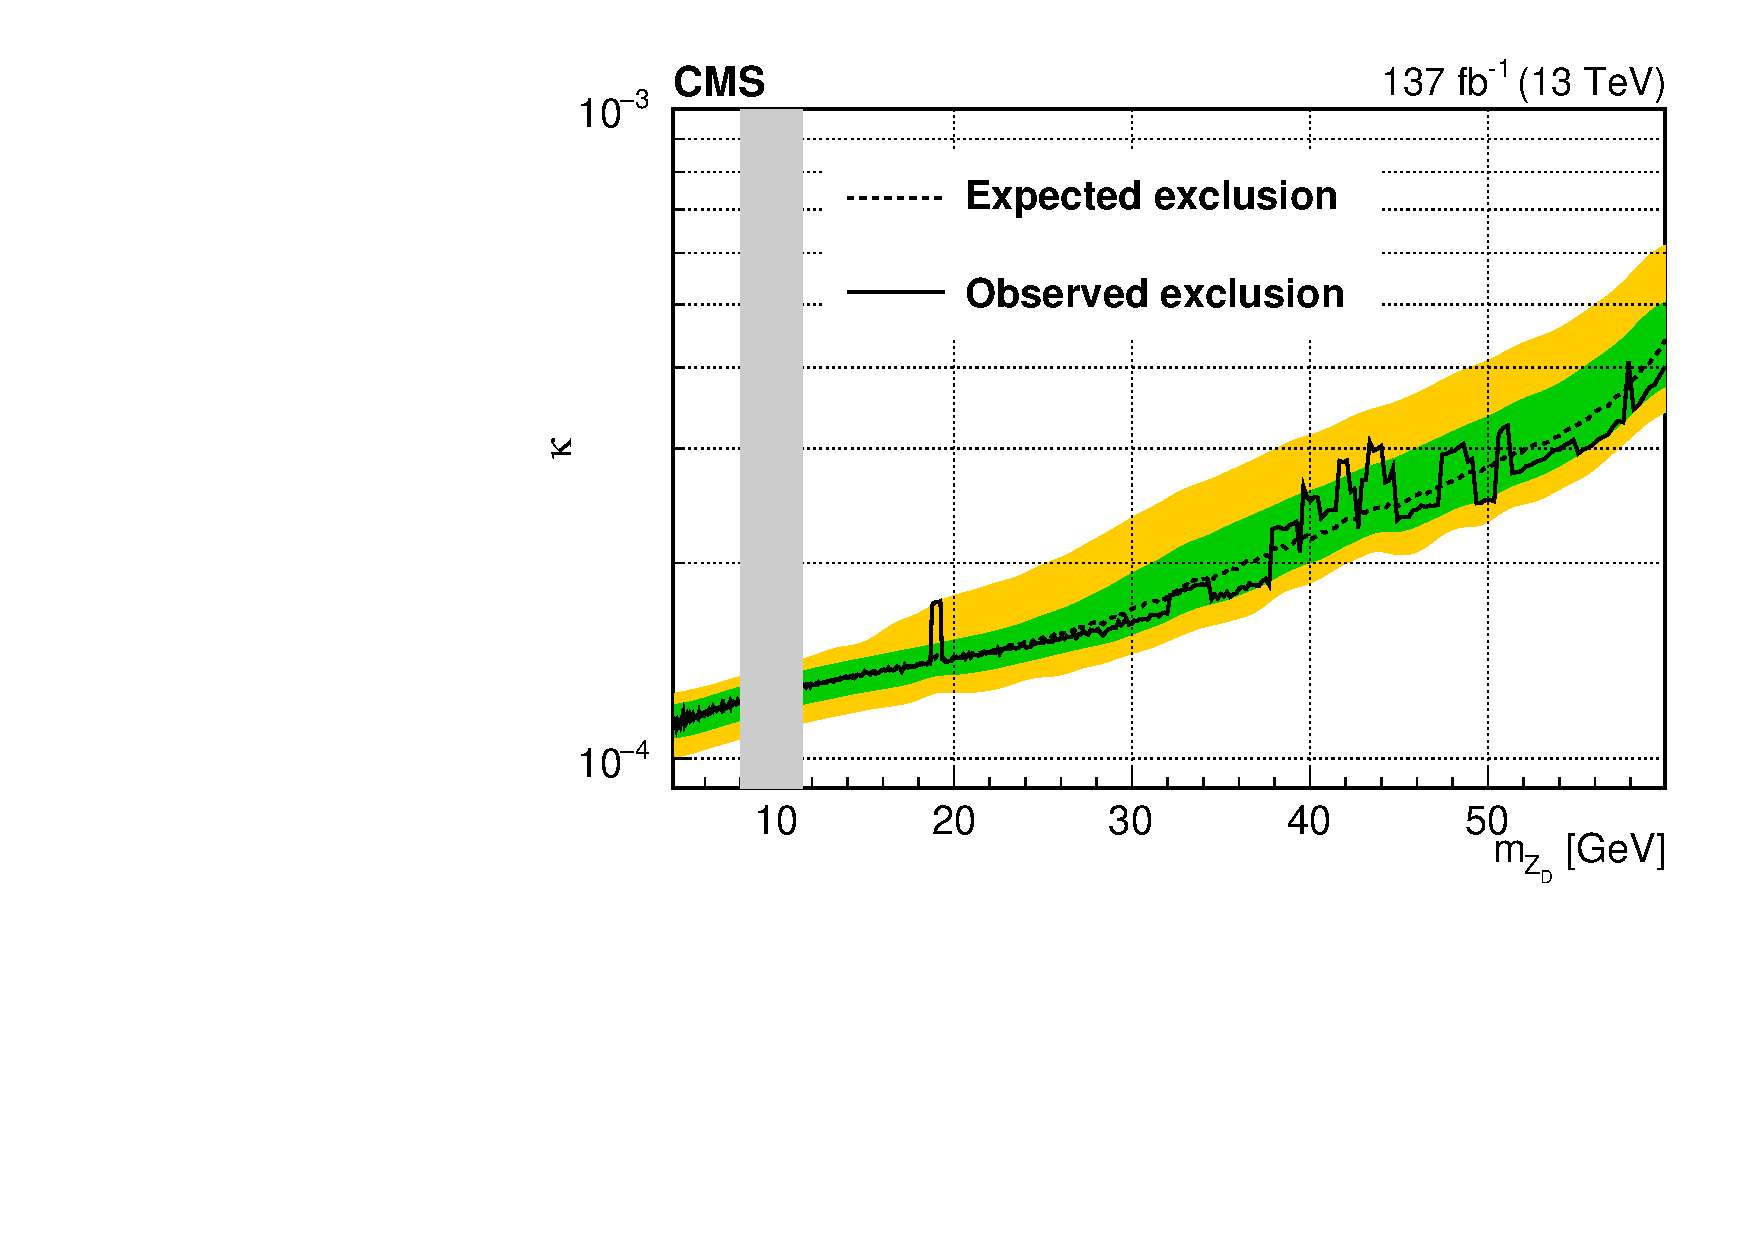
\includegraphics[width=0.48\textwidth]{figures/dilep_res/exclus_lim_kappa.pdf}
    \captionof{figure}
        [Expected and observed exclusion limits on the Higgs-mixing parameter] % TODO: ?
        {Expected and observed exclusion limits on the Higgs-mixing parameter.} % TODO: ?
    \label{fig:exclus_lim_kappa}
\end{multiFigure}

